\documentclass{article}

\usepackage{physics}
\usepackage{amsmath}
\usepackage{tikz}
\usepackage{mathdots}
\usepackage{yhmath}
\usepackage{cancel}
\usepackage{color}
\usepackage{siunitx}
\usepackage{array}
\usepackage{multirow}
\usepackage{amssymb}
\usepackage{gensymb}
\usepackage{tabularx}
\usepackage{extarrows}
\usepackage{booktabs}
\usetikzlibrary{fadings}
\usetikzlibrary{patterns}
\usetikzlibrary{shadows.blur}
\usetikzlibrary{shapes}




% set font encoding for PDFLaTeX, XeLaTeX, or LuaTeX
\usepackage{ifxetex,ifluatex}
\if\ifxetex T\else\ifluatex T\else F\fi\fi T%
  \usepackage{fontspec}
\else
  \usepackage[T1]{fontenc}
  \usepackage[utf8]{inputenc}
  \usepackage{lmodern}
\fi

\usepackage{hyperref, amssymb, amsmath, multicol, graphicx, paracol}

\usepackage[margin=0.8in]{geometry}

\pagenumbering{gobble}


\newcommand{\R}{\mathbb{R}}


\begin{document}


\begin{center}
\begin{Huge}Pre-Calculus Exercises\end{Huge}
\end{center}


\subsection*{A. Prove the following identities.}
\begin{multicols}{3}
\begin{enumerate}
    \item $\tan(x+y)=\frac{\tan(x)+\tan(y)}{1-\tan(x)\tan(y)}$
    \item $\sin(3x)=3\sin(x)-4\sin(x)^3$
    \item $\cos(x)\cos(y)=\frac{\cos(x-y)+\cos(x+y)}{2}$
\end{enumerate}
\end{multicols}

\subsection*{B. Refer to the diagram of the triangle. Find the indicated value for each given set of angle and side measurements.}

\begin{multicols}{2}

\tikzset{every picture/.style={line width=0.75pt}} %set default line width to 0.75pt        

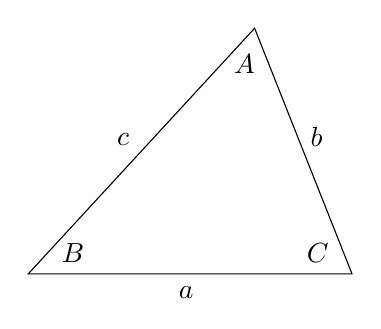
\begin{tikzpicture}[x=0.75pt,y=0.75pt,yscale=-1,xscale=1]
%uncomment if require: \path (0,440); %set diagram left start at 0, and has height of 440

%Shape: Triangle [id:dp38838544803006925] 
\draw   (204.07,67.67) -- (251,186.04) -- (95,186.04) -- cycle ;

% Text Node
\draw (166.34,190.96) node [anchor=north west][inner sep=0.75pt]    {$a$};
% Text Node
\draw (229.8,114.08) node [anchor=north west][inner sep=0.75pt]    {$b$};
% Text Node
\draw (136.59,117.13) node [anchor=north west][inner sep=0.75pt]    {$c$};
% Text Node
\draw (192.93,79.3) node [anchor=north west][inner sep=0.75pt]    {$A$};
% Text Node
\draw (228,170) node [anchor=north west][inner sep=0.75pt]    {$C$};
% Text Node
\draw (110,170) node [anchor=north west][inner sep=0.75pt]    {$B$};


\end{tikzpicture}

\columnbreak

\begin{enumerate}
    \item $a=6$, $B=\pi/2$, $A=\pi/4$, $c=?$
    \item $a=1$, $b=1$, $C=\pi/3$, $c=?$
    \item $A=\pi/2$, $b=3$, $C=\pi/4$, $a=?$
    \item $C=\pi/2$, $a=1$, $b=1$, $c=?$
    \item $a=b=c=1$, $A=?$
\end{enumerate}
\end{multicols}


\subsection*{C. Draw the following sets on a number line.}
\begin{multicols}{3}
\begin{enumerate}
    \item $(0,3)\cup (4,6)$
    \item $[0,5]\cap (1, 10]$
    \item $\{2x\ :\ x\in \R\}\cap(0,10)$
    \item $\{x^2\ :\ x\in\R\}\cup(0,1)$
    \item $\{x\in\R\ :\ x^2-4<0\}$
    \item $\{x\in\R\ :\ x^2 > 0\}$
\end{enumerate}

\end{multicols}


\subsection*{D. For each real-function, state the (largest possible) domain and range. State whether the function is injective, surjective, and/or bijective. Then find a restricted domain and codomain on which the function is invertible, and find its inverse.}
\begin{multicols}{3}
\begin{enumerate}
    \item $f(x)=\sqrt{x}$
    \item $f(x)=x^3$
    \item $f(x)=x^4$
    \item $f(x)=\frac{1}{x+1}$
    \item $f(x)=\frac{x}{x^2+x}$
    \item $f(x)=\cos(x)$
    \item $f(x)=\tan(x)$
    \item $f(x)=\csc(x)$
    \item $f(x)=\log_2(x)$
\end{enumerate}
\end{multicols}



\end{document}
